% !TEX program = xelatex
% Biên dịch: xelatex main.tex (chạy 2 lần để cập nhật mục lục & tham chiếu)
\RequirePackage{fix-cm}
\documentclass[a4paper]{article}

% ---------- Cỡ chữ 13pt thật sự (lớp report chuẩn chỉ hỗ trợ 10/11/12pt,
% nên option [13pt] bị bỏ qua; gói fontsize cho phép đặt cỡ tuỳ ý) ----------
\usepackage[fontsize=13pt]{fontsize}

% ---------- Ngôn ngữ & font (XeLaTeX) ----------
\usepackage{fontspec}
\usepackage{amsmath}
\usepackage{amssymb}
\usepackage{unicode-math}
\usepackage{polyglossia}
\setdefaultlanguage{vietnamese}
% Font Latin Modern (font TeX cổ điển) — giống bài mẫu, có hỗ trợ tiếng Việt
\setmainfont{Latin Modern Roman}
\setmathfont{Latin Modern Math}
% LM Mono không có bản bold → ánh xạ bold về regular để tránh cảnh báo font
\setmonofont{Latin Modern Mono}[BoldFont={Latin Modern Mono}]

% ---------- Trình bày trang ----------
\usepackage[a4paper,left=3.5cm,right=2cm,top=2.5cm,bottom=2.5cm]{geometry}
\usepackage{setspace}
\onehalfspacing
% Cho phép TeX nới dòng ở bước cuối để tránh text tràn lề (overfull hbox)
\setlength{\emergencystretch}{3em}
% Bỏ qua các cảnh báo underfull nhẹ do tiếng Việt và tên vùng dài trong danh sách.
\hbadness=2000

% ---------- Hình, bảng, biểu ----------
\usepackage{graphicx}
\graphicspath{{figures/}}
\usepackage{float}
\usepackage{booktabs}
\usepackage{longtable}
\usepackage{array}
\usepackage{multirow}
\usepackage{makecell}
\usepackage[font=small,labelfont=bf]{caption}
\usepackage{subcaption}
\usepackage[table]{xcolor}

% ---------- Sơ đồ minh hoạ ----------
\usepackage{tikz}
\usetikzlibrary{arrows.meta,positioning,shapes.geometric,calc}

% ---------- Liên kết ----------
\usepackage[hidelinks]{hyperref}
\usepackage{enumitem}

% \code: định danh dạng monospace; cho phép ngắt dòng ngay sau dấu gạch dưới
% để các tên biến dài (vd. num_of_prev_attempts) không tràn ra lề.
\newcommand{\code}[1]{{\ttfamily\def\_{\textunderscore\discretionary{}{}{}}#1}}
\pdfstringdefDisableCommands{%
  \def\code#1{#1}%
  \def\_{ }%
}

\begin{document}

% =====================================================================
%  TRANG BÌA
% =====================================================================
\begin{titlepage}
  \centering
  {\large\bfseries TRƯỜNG ĐẠI HỌC QUY NHƠN\\[3pt]
   KHOA TOÁN \& THỐNG KÊ\par}

  \vspace{1.3cm}

  % ----- LOGO trường -----
  
\includegraphics[width=3.5cm]{logo_qnu.png}\par

  \vspace{1.4cm}

  {\bfseries TIỂU LUẬN MÔN HỌC:\\[3pt]
   PHÂN TÍCH DỮ LIỆU KHOA HỌC CHUYÊN NGÀNH\par}

  \vspace{0.5cm}
  \rule{\textwidth}{0.4pt}\\[0.55cm]
  {\LARGE\bfseries CƠ SỞ LÝ THUYẾT CÁC THUẬT TOÁN\\[6pt]
   HỌC MÁY SỬ DỤNG TRONG BÀI TOÁN\\[6pt]
   CẢNH BÁO SỚM RỦI RO HỌC TẬP\par}
  \vspace{0.5cm}
  \rule{\textwidth}{0.4pt}

  \vspace{2.4cm}

  {\normalsize
  \begin{tabular}{r@{\hspace{0.5em}}l}
    \itshape Trình độ đào tạo:      & Thạc sĩ \\[5pt]
    \itshape Học viên thực hiện:    & Nguyễn Hồ Bảo Thiên \\[5pt]
    \itshape Mã số sinh viên:       & 8282548017 \\[5pt]
    \itshape Lớp:                   & Khoa học dữ liệu K28B \\[5pt]
    \itshape Giảng viên hướng dẫn:  & TS. Hồ Văn Lâm \\
  \end{tabular}\par}

  \vfill
  {\itshape Gia Lai, 2026\par}
\end{titlepage}

% =====================================================================
%  PHẦN ĐẦU (mục lục, danh mục hình/bảng) — đánh số La Mã
% =====================================================================
\pagenumbering{roman}
\tableofcontents
\listoffigures
\listoftables
\clearpage

% =====================================================================
%  NỘI DUNG CHÍNH — đánh số Ả Rập
% =====================================================================
\pagenumbering{arabic}

\section{Giới thiệu}

Báo cáo này trình bày cơ sở lý thuyết của bốn thuật toán học máy được lựa chọn
để xây dựng và so sánh mô hình cho bài toán \textit{cảnh báo sớm rủi ro học
tập}: \textbf{Logistic Regression}, \textbf{Random Forest}, \textbf{CatBoost}
và \textbf{LightGBM}. Đây là các thuật toán đã được đề xuất dựa trên đặc điểm
dữ liệu quan sát được ở giai đoạn phân tích khám phá dữ liệu (EDA) --- dữ liệu
dạng bảng, mất cân bằng nhãn, có cả đặc trưng phân loại lẫn đặc trưng số, tồn
tại quan hệ phi tuyến và đa cộng tuyến giữa một số nhóm đặc trưng --- và được
sử dụng trực tiếp ở giai đoạn xây dựng và so sánh mô hình.

Bốn thuật toán này đại diện cho ba trường phái tiếp cận khác nhau trong học
máy có giám sát:

\begin{itemize}[leftmargin=*]
  \item \textbf{Mô hình tuyến tính} (Logistic Regression) --- đơn giản, dễ
        diễn giải, làm cơ sở đối chiếu (baseline).
  \item \textbf{Học tập hợp dạng bagging} (Random Forest) --- tổng hợp nhiều
        cây quyết định độc lập để giảm phương sai.
  \item \textbf{Học tập hợp dạng boosting} (CatBoost, LightGBM) --- xây dựng
        tuần tự nhiều mô hình yếu để giảm sai số một cách có hệ thống, với hai
        cách hiện thực hoá khác nhau.
\end{itemize}

Với mỗi thuật toán, báo cáo trình bày: nguyên lý hoạt động, công thức toán học
cốt lõi, các cơ chế đặc trưng riêng (nếu có), và phân tích ưu điểm --- hạn chế
trong bối cảnh bài toán cảnh báo sớm. Phần cuối tổng hợp một bảng so sánh
xuyên suốt bốn thuật toán theo nhiều tiêu chí thực tiễn.

\section{Hồi quy Logistic (Logistic Regression)}

\subsection{Mô hình xác suất}

Logistic Regression là một mô hình \textbf{tuyến tính suy rộng} (generalized
linear model) cho bài toán phân loại nhị phân. Với vector đặc trưng đầu vào
$\mathbf{x} \in \mathbb{R}^p$, mô hình trước tiên tính một tổ hợp tuyến tính:

\[
  z = \mathbf{w}^\top \mathbf{x} + b,
\]

trong đó $\mathbf{w} \in \mathbb{R}^p$ là vector trọng số và $b$ là hệ số chặn
(bias). Giá trị $z$ sau đó được ánh xạ về khoảng $(0, 1)$ thông qua \textbf{hàm
sigmoid}:

\[
  \hat{p} = \sigma(z) = \frac{1}{1 + e^{-z}},
\]

được diễn giải là xác suất dự báo của lớp dương (ở đây là At-risk). Quyết định
phân loại cuối cùng dựa trên một ngưỡng $\tau$ (mặc định $\tau = 0.5$):
$\hat{y} = 1$ nếu $\hat{p} \ge \tau$, ngược lại $\hat{y} = 0$.

\begin{figure}[H]
  \centering
  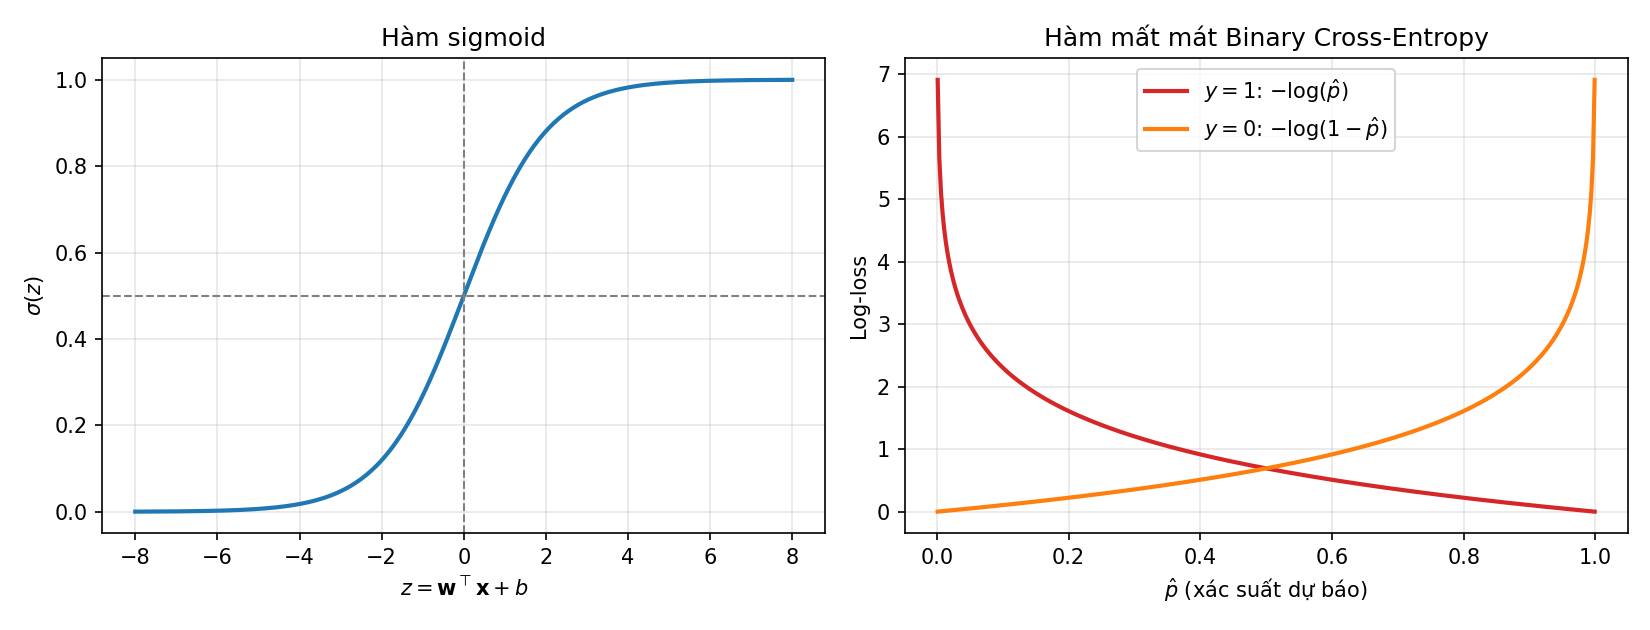
\includegraphics[width=0.95\textwidth]{sigmoid_logloss.png}
  \caption{Hàm sigmoid (trái) và hàm mất mát Binary Cross-Entropy theo xác
  suất dự báo, ứng với hai trường hợp nhãn thật $y=1$ và $y=0$ (phải).}
  \label{fig:sigmoid}
\end{figure}

Như minh hoạ ở Hình~\ref{fig:sigmoid} (trái), hàm sigmoid có dạng chữ S, đối
xứng qua điểm $(0, 0.5)$, bão hoà dần về 0 và 1 ở hai đầu --- đây chính là cơ
chế giúp mô hình tuyến tính $z$ (có thể nhận giá trị bất kỳ trên
$\mathbb{R}$) được chuyển thành một xác suất hợp lệ.

\subsection{Hàm mất mát và ước lượng tham số}

Tham số $(\mathbf{w}, b)$ được ước lượng bằng phương pháp \textbf{hợp lý cực
đại} (Maximum Likelihood Estimation), tương đương với việc tối thiểu hoá hàm
mất mát \textbf{Binary Cross-Entropy} (hay log-loss) trên tập huấn luyện gồm
$N$ mẫu:

\[
  \mathcal{L}(\mathbf{w}, b) = -\frac{1}{N} \sum_{i=1}^{N}
  \Big[ y_i \log(\hat{p}_i) + (1 - y_i) \log(1 - \hat{p}_i) \Big].
\]

Hình~\ref{fig:sigmoid} (phải) minh hoạ trực quan hàm mất mát này: khi nhãn
thật $y_i = 1$, mất mát giảm dần về 0 khi $\hat{p}_i \to 1$ nhưng tiến tới vô
cực khi $\hat{p}_i \to 0$ --- tức mô hình bị phạt rất nặng nếu dự báo sai với
độ tin cậy cao. Vì $\mathcal{L}$ là hàm lồi theo $(\mathbf{w}, b)$, việc tối ưu
thường dùng các phương pháp lặp dựa trên gradient (gradient descent hoặc các
biến thể tựa Newton như L-BFGS), với đạo hàm riêng theo $\mathbf{w}$ có dạng
tường minh:

\[
  \nabla_{\mathbf{w}} \mathcal{L} = \frac{1}{N} \mathbf{X}^\top
  (\hat{\mathbf{p}} - \mathbf{y}).
\]

\subsection{Điều chuẩn (Regularization)}

Để hạn chế hiện tượng học vẹt (overfitting) khi số đặc trưng lớn hoặc các đặc
trưng có tương quan mạnh, một số hạng điều chuẩn được cộng thêm vào hàm mục
tiêu. Với điều chuẩn $L_2$ (Ridge), bài toán tối ưu trở thành:

\[
  \min_{\mathbf{w}, b} \; \frac{1}{2} \lVert \mathbf{w} \rVert_2^2
  + C \sum_{i=1}^{N} \ell(y_i, \hat{p}_i),
\]

trong đó $\ell$ là hàm mất mát log-loss của từng mẫu, và $C > 0$ là siêu tham
số \textbf{nghịch đảo} của cường độ điều chuẩn: $C$ càng nhỏ, mô hình bị ràng
buộc càng chặt (trọng số $\mathbf{w}$ bị co về gần 0), giảm phương sai nhưng có
thể tăng độ chệch (bias); $C$ càng lớn, mô hình càng tự do khớp dữ liệu huấn
luyện. Đây chính là siêu tham số $C$ được tinh chỉnh bằng Optuna ở giai đoạn
xây dựng mô hình.

\subsection{Trọng số lớp cho dữ liệu mất cân bằng}

Với bài toán mất cân bằng nhãn, hàm mất mát có thể được điều chỉnh bằng cách
gán trọng số khác nhau cho từng lớp:

\[
  \mathcal{L}_w(\mathbf{w}, b) = -\frac{1}{N} \sum_{i=1}^{N} w_{y_i}
  \Big[ y_i \log(\hat{p}_i) + (1 - y_i) \log(1 - \hat{p}_i) \Big],
\]

trong đó $w_{y_i}$ là trọng số ứng với lớp của mẫu $i$ (thường $w_0 = 1$ và
$w_1 > 1$ cho lớp thiểu số At-risk). Việc tăng $w_1$ khiến mô hình phải trả giá
mất mát lớn hơn khi phân loại sai một sinh viên At-risk, thúc đẩy mô hình dịch
chuyển ranh giới quyết định để bắt được nhiều trường hợp At-risk hơn --- đây
chính là cơ chế \code{class\_weight} được tinh chỉnh đồng thời với $C$ và tỷ lệ
SMOTE trong các thử nghiệm.

\subsection{Ưu điểm và hạn chế}

\textbf{Ưu điểm:}
\begin{itemize}[leftmargin=*]
  \item Đơn giản, huấn luyện nhanh, phù hợp làm mô hình cơ sở để đối chiếu với
        các mô hình phức tạp hơn.
  \item Khả năng diễn giải cao: dấu và độ lớn của từng trọng số $w_j$ (trên dữ
        liệu đã chuẩn hoá) cho biết chiều và mức độ ảnh hưởng của đặc trưng
        tương ứng đến nguy cơ At-risk.
  \item Đầu ra là xác suất được hiệu chỉnh tốt (well-calibrated) trong nhiều
        trường hợp, thuận lợi cho việc điều chỉnh ngưỡng cảnh báo theo nhu cầu
        thực tế.
\end{itemize}

\textbf{Hạn chế:}
\begin{itemize}[leftmargin=*]
  \item Ranh giới quyết định về bản chất là một siêu phẳng tuyến tính trong
        không gian đặc trưng, nên khó nắm bắt quan hệ phi tuyến và tương tác
        giữa các đặc trưng, trừ khi tự thêm số hạng tương tác thủ công.
  \item Nhạy cảm với đa cộng tuyến --- khi hai đặc trưng tương quan cao, ma
        trận $\mathbf{X}^\top \mathbf{X}$ gần suy biến, khiến hệ số ước lượng
        bất ổn và khó diễn giải.
  \item Nhạy với thang đo của đặc trưng, bắt buộc phải chuẩn hoá dữ liệu số
        trước khi huấn luyện.
  \item Không tự xử lý được giá trị thiếu hay đặc trưng phân loại; cần điền
        khuyết và mã hoá thủ công trước khi đưa vào mô hình.
\end{itemize}

\section{Cây quyết định và Random Forest}

\subsection{Cây quyết định (Decision Tree)}

Cây quyết định (cụ thể là thuật toán CART --- Classification and Regression
Tree) xây dựng mô hình bằng cách chia đệ quy không gian đặc trưng thành các
vùng ngày càng nhỏ, mỗi vùng ứng với một \textbf{lá} (leaf) mang một dự báo cụ
thể. Tại mỗi nút, thuật toán chọn một đặc trưng $j$ và một ngưỡng $s$ sao cho
việc chia dữ liệu thành hai nhánh $\{\mathbf{x} : x_j \le s\}$ và
$\{\mathbf{x} : x_j > s\}$ làm giảm nhiều nhất một độ đo \textbf{tạp chất}
(impurity). Với bài toán phân loại, độ đo phổ biến nhất là chỉ số
\textbf{Gini}:

\[
  \text{Gini}(t) = 1 - \sum_{k} p_k(t)^2,
\]

trong đó $p_k(t)$ là tỷ lệ mẫu thuộc lớp $k$ tại nút $t$. Gini$(t) = 0$ khi nút
$t$ hoàn toàn thuần nhất (chỉ chứa một lớp), và đạt giá trị lớn nhất khi các
lớp phân bố đều. Độ giảm tạp chất khi chia nút $t$ thành hai nút con
$t_L, t_R$ là:

\[
  \Delta \text{Gini} = \text{Gini}(t) - \frac{N_L}{N_t}\text{Gini}(t_L)
  - \frac{N_R}{N_t}\text{Gini}(t_R),
\]

và thuật toán chọn cặp $(j, s)$ tối đa hoá $\Delta \text{Gini}$ tại mỗi nút.
Quá trình chia dừng lại khi đạt điều kiện dừng (độ sâu tối đa, số mẫu tối
thiểu mỗi lá, hoặc tạp chất bằng 0).

\begin{figure}[H]
  \centering
  \resizebox{\textwidth}{!}{%
  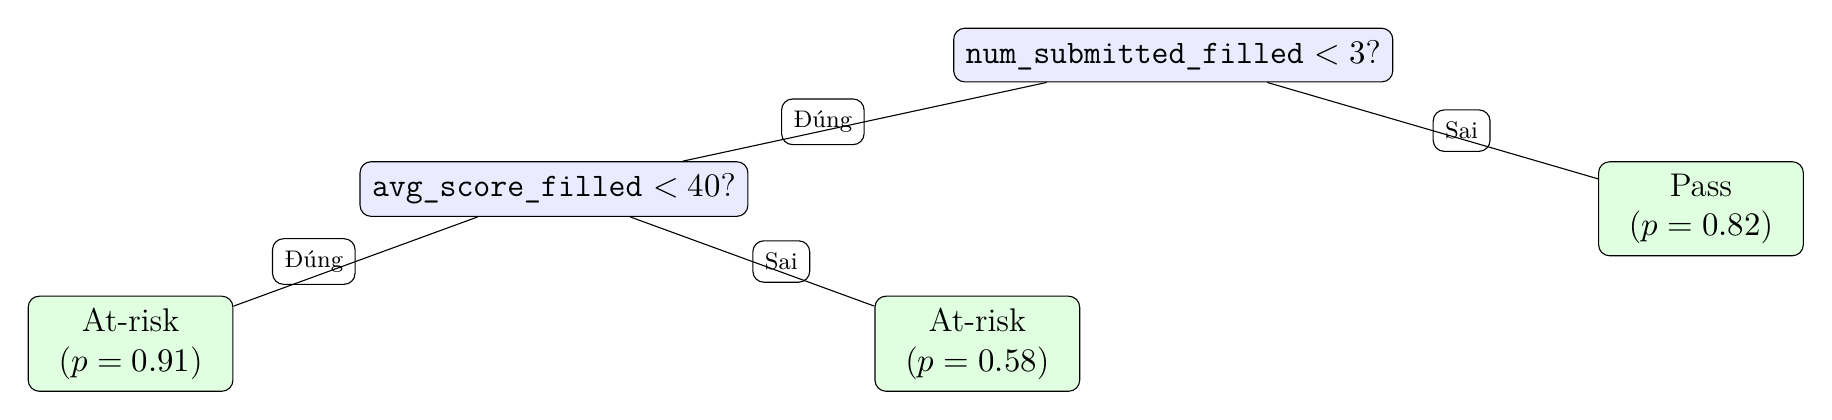
\begin{tikzpicture}[
      level distance=15mm,
      every node/.style={draw, rounded corners, align=center, font=\small},
      internal/.style={fill=blue!8, minimum width=3.6cm},
      leaf/.style={fill=green!12, minimum width=2.6cm},
      edge label/.style={font=\scriptsize, midway}
    ]
    \node[internal] (root) {\code{num\_submitted\_filled} $< 3$?};
    \node[internal, below left=of root, xshift=-1.6cm] (n1) {\code{avg\_score\_filled} $< 40$?};
    \node[leaf, below right=of root, xshift=1.6cm] (n2) {Pass\\($p=0.82$)};
    \node[leaf, below left=of n1, xshift=-0.6cm] (n3) {At-risk\\($p=0.91$)};
    \node[leaf, below right=of n1, xshift=0.6cm] (n4) {At-risk\\($p=0.58$)};

    \draw (root) -- node[edge label, left] {Đúng} (n1);
    \draw (root) -- node[edge label, right] {Sai} (n2);
    \draw (n1) -- node[edge label, left] {Đúng} (n3);
    \draw (n1) -- node[edge label, right] {Sai} (n4);
  \end{tikzpicture}}
  \caption{Ví dụ minh hoạ một cây quyết định nông (2 tầng) trên các đặc trưng
  của bài toán cảnh báo sớm. Giá trị $p$ trong mỗi lá là xác suất At-risk ước
  lượng từ tỷ lệ mẫu huấn luyện rơi vào lá đó.}
  \label{fig:tree}
\end{figure}

Cây quyết định đơn lẻ có ưu điểm diễn giải trực quan (Hình~\ref{fig:tree}) và
tự nhiên xử lý được cả đặc trưng số lẫn phân loại, nhưng có \textbf{phương sai
rất cao}: chỉ cần thay đổi nhỏ trong dữ liệu huấn luyện cũng có thể dẫn đến một
cấu trúc cây hoàn toàn khác, dễ học vẹt nếu để cây phát triển quá sâu.

\subsection{Bagging (Bootstrap Aggregating)}

Để giảm phương sai của cây quyết định, \textbf{bagging} huấn luyện nhiều cây
độc lập trên các tập dữ liệu được lấy mẫu lại (bootstrap) từ tập huấn luyện
gốc, rồi tổng hợp kết quả dự báo.

\begin{figure}[H]
  \centering
  \resizebox{\textwidth}{!}{%
  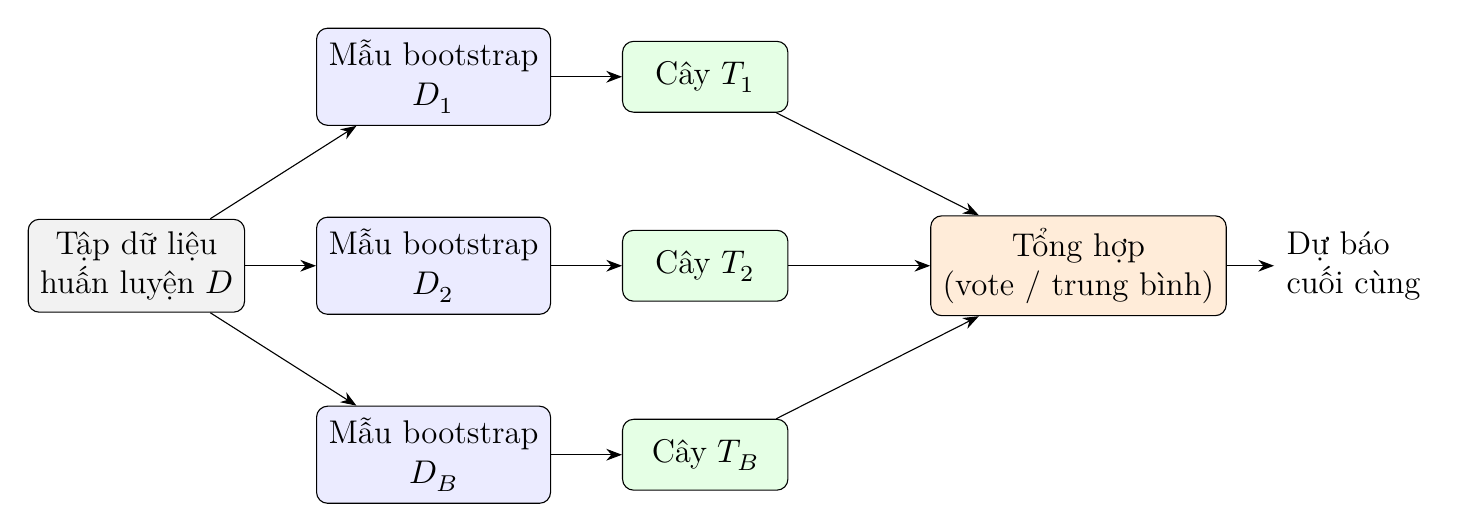
\begin{tikzpicture}[
      node distance=6mm and 9mm,
      box/.style={draw, rounded corners, align=center, font=\small, minimum width=2.1cm, minimum height=0.9cm},
      >={Stealth[length=2mm]}
    ]
    \node[box, fill=gray!10] (D) {Tập dữ liệu\\huấn luyện $D$};

    \node[box, fill=blue!8, right=of D, yshift=2.4cm] (b1) {Mẫu bootstrap\\$D_1$};
    \node[box, fill=blue!8, right=of D] (b2) {Mẫu bootstrap\\$D_2$};
    \node[box, fill=blue!8, right=of D, yshift=-2.4cm] (b3) {Mẫu bootstrap\\$D_B$};

    \node[box, fill=green!10, right=of b1] (t1) {Cây $T_1$};
    \node[box, fill=green!10, right=of b2] (t2) {Cây $T_2$};
    \node[box, fill=green!10, right=of b3] (t3) {Cây $T_B$};

    \node[box, fill=orange!15, right=18mm of t2] (agg) {Tổng hợp\\(vote / trung bình)};

    \draw[->] (D) -- (b1);
    \draw[->] (D) -- (b2);
    \draw[->] (D) -- (b3);
    \draw[->] (b1) -- (t1);
    \draw[->] (b2) -- (t2);
    \draw[->] (b3) -- (t3);
    \draw[->] (t1) -- (agg);
    \draw[->] (t2) -- (agg);
    \draw[->] (t3) -- (agg);

    \node[right=6mm of agg, align=left, font=\small] (out) {Dự báo\\cuối cùng};
    \draw[->] (agg) -- (out);
  \end{tikzpicture}}
  \caption{Sơ đồ nguyên lý Bagging: $B$ cây được huấn luyện độc lập trên các
  mẫu bootstrap khác nhau, kết quả được tổng hợp bằng biểu quyết đa số (phân
  loại) hoặc trung bình (hồi quy).}
  \label{fig:bagging}
\end{figure}

Mỗi mẫu bootstrap $D_b$ ($b = 1, \ldots, B$) có cùng kích thước với $D$ nhưng
được lấy \textbf{có hoàn lại}, nên trung bình khoảng 63.2\% số mẫu gốc xuất
hiện trong mỗi $D_b$ (một số mẫu lặp lại, một số không xuất hiện). Với bài
toán phân loại, dự báo cuối cùng là lớp chiếm đa số trong $B$ dự báo:

\[
  \hat{y}(\mathbf{x}) = \text{mode}\big\{ T_1(\mathbf{x}), T_2(\mathbf{x}),
  \ldots, T_B(\mathbf{x}) \big\}.
\]

Vì các cây được huấn luyện trên các mẫu khác nhau nên sai số của chúng có xu
hướng \textbf{không tương quan hoàn toàn}; việc lấy trung bình/biểu quyết giúp
triệt tiêu bớt nhiễu ngẫu nhiên, giảm phương sai tổng thể mà không làm tăng
đáng kể độ chệch.

\subsection{Random Forest}

Random Forest cải tiến bagging bằng cách thêm một nguồn ngẫu nhiên hoá thứ
hai: tại \textbf{mỗi nút} của mỗi cây, thay vì xét toàn bộ $p$ đặc trưng để tìm
điểm chia tốt nhất, thuật toán chỉ xét một tập con ngẫu nhiên gồm
$m < p$ đặc trưng (thường $m \approx \sqrt{p}$ cho bài toán phân loại). Cơ chế
này \textbf{decorrelate} (giảm tương quan) giữa các cây: nếu không có bước
này, các cây bagging vẫn có xu hướng chọn cùng một vài đặc trưng mạnh nhất ở
gần gốc, khiến chúng giống nhau và hạn chế hiệu quả giảm phương sai.

\subsection{Độ quan trọng đặc trưng}

Random Forest cung cấp một thước đo độ quan trọng đặc trưng dựa trên tổng độ
giảm tạp chất (Mean Decrease in Impurity):

\[
  \text{Importance}(x_j) = \frac{1}{B} \sum_{b=1}^{B} \;
  \sum_{t \in T_b : \, \text{split trên } x_j} \frac{N_t}{N} \Delta\text{Gini}(t),
\]

tức trung bình cộng (qua toàn bộ $B$ cây) tổng mức giảm Gini tại các nút sử
dụng đặc trưng $x_j$ để chia, có trọng số theo tỷ lệ mẫu đi qua nút đó. Đây là
thước đo \code{feature\_importances\_} mặc định của Random Forest trong
scikit-learn.

\subsection{Ưu điểm và hạn chế}

\textbf{Ưu điểm:}
\begin{itemize}[leftmargin=*]
  \item Tự nắm bắt quan hệ phi tuyến và tương tác giữa các đặc trưng mà không
        cần khai báo thủ công.
  \item Bền vững với giá trị ngoại lai và không yêu cầu chuẩn hoá dữ liệu.
  \item Cơ chế tổng hợp nhiều cây giúp giảm phương sai, hạn chế học vẹt so với
        một cây đơn lẻ; đồng thời cung cấp thước đo độ quan trọng đặc trưng.
\end{itemize}

\textbf{Hạn chế:}
\begin{itemize}[leftmargin=*]
  \item Mô hình cồng kềnh (gồm $B$ cây), tốc độ dự báo chậm hơn và khó diễn
        giải chi tiết so với hồi quy tuyến tính.
  \item Với dữ liệu mất cân bằng, cần kết hợp thêm trọng số lớp hoặc kỹ thuật
        lấy mẫu lại mới nhận diện tốt nhóm thiểu số.
  \item Không hỗ trợ xử lý giá trị thiếu trực tiếp trong hầu hết cài đặt phổ
        biến (như scikit-learn). Đặc trưng tương quan mạnh cũng làm sai lệch
        thước đo độ quan trọng --- tầm quan trọng thực sự bị ``chia sẻ'' giữa
        các đặc trưng tương quan với nhau.
\end{itemize}

\section{Gradient Boosting và CatBoost}
\label{sec:catboost}

\subsection{Nguyên lý Gradient Boosting}

Khác với bagging (huấn luyện các cây \textbf{độc lập} rồi tổng hợp), boosting
xây dựng mô hình theo kiểu \textbf{tuần tự} (additive): mỗi cây mới được huấn
luyện để sửa chữa sai số của tổ hợp các cây trước đó. Gọi $F_m(\mathbf{x})$ là
mô hình tổng hợp sau $m$ vòng, gradient boosting cập nhật:

\[
  F_m(\mathbf{x}) = F_{m-1}(\mathbf{x}) + \eta \, h_m(\mathbf{x}),
\]

trong đó $\eta \in (0, 1]$ là tốc độ học (learning rate) và $h_m$ là một cây
quyết định yếu (thường nông, vài tầng), được huấn luyện để xấp xỉ
\textbf{gradient âm} của hàm mất mát tại $F_{m-1}$ --- gọi là \textbf{giả
phần dư} (pseudo-residual):

\[
  r_i^{(m)} = -\left[ \frac{\partial \, \ell(y_i, F(\mathbf{x}_i))}
  {\partial \, F(\mathbf{x}_i)} \right]_{F = F_{m-1}}.
\]

Với hàm mất mát log-loss (như ở Logistic Regression), giả phần dư có dạng đơn
giản $r_i^{(m)} = y_i - \hat{p}_i^{(m-1)}$ --- tức phần chênh lệch giữa nhãn
thật và xác suất dự báo hiện tại. Cây $h_m$ được huấn luyện để dự báo chính
các giả phần dư này, và mô hình dần được "sửa lỗi" qua từng vòng lặp.

\begin{figure}[H]
  \centering
  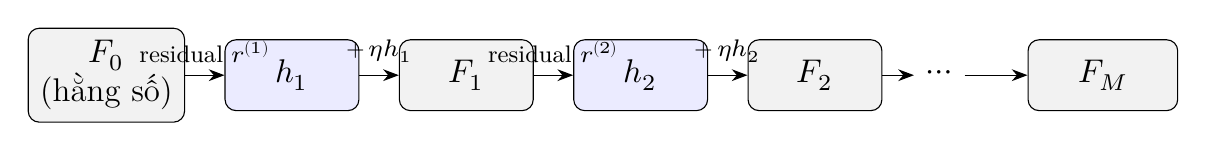
\begin{tikzpicture}[
      node distance=5mm,
      box/.style={draw, rounded corners, align=center, font=\small, minimum height=0.9cm},
      >={Stealth[length=2mm]}
    ]
    \node[box, fill=gray!10, minimum width=1.7cm] (f0) {$F_0$\\(hằng số)};
    \node[box, fill=blue!8, right=of f0, minimum width=1.7cm] (h1) {$h_1$};
    \node[box, fill=gray!10, right=of h1, minimum width=1.7cm] (f1) {$F_1$};
    \node[box, fill=blue!8, right=of f1, minimum width=1.7cm] (h2) {$h_2$};
    \node[box, fill=gray!10, right=of h2, minimum width=1.7cm] (f2) {$F_2$};
    \node[right=4mm of f2, font=\small] (dots) {$\cdots$};
    \node[box, fill=gray!10, right=8mm of dots, minimum width=1.9cm] (fm) {$F_M$};

    \draw[->] (f0) -- node[above, font=\scriptsize] {residual $r^{(1)}$} (h1);
    \draw[->] (h1) -- node[above, font=\scriptsize] {$+\,\eta h_1$} (f1);
    \draw[->] (f1) -- node[above, font=\scriptsize] {residual $r^{(2)}$} (h2);
    \draw[->] (h2) -- node[above, font=\scriptsize] {$+\,\eta h_2$} (f2);
    \draw[->] (f2) -- (dots);
    \draw[->] (dots) -- (fm);
  \end{tikzpicture}
  \caption{Sơ đồ boosting tuần tự: mỗi cây yếu $h_m$ được huấn luyện để dự báo
  giả phần dư của mô hình tổng hợp ở vòng trước, sau đó được cộng dồn (có
  trọng số $\eta$) vào mô hình.}
  \label{fig:boosting}
\end{figure}

CatBoost và LightGBM đều thuộc họ \textbf{Gradient Boosted Decision Trees}
(GBDT) --- dùng cây quyết định làm bộ học yếu $h_m$ --- nhưng khác nhau đáng
kể ở cách hiện thực hoá nhằm giải quyết các nhược điểm cố hữu của GBDT
truyền thống, được trình bày ở các mục tiếp theo.

\subsection{Ordered Boosting}

Một vấn đề tinh vi của GBDT truyền thống là \textbf{prediction shift}
(lệch dự báo, hay rò rỉ mục tiêu): giả phần dư $r_i^{(m)}$ của một mẫu
$\mathbf{x}_i$ được tính từ mô hình $F_{m-1}$ vốn \textbf{đã được huấn luyện
trên chính mẫu đó} ở các vòng trước, khiến giả phần dư bị chệch (thiên lệch
lạc quan) so với giả phần dư thật sự trên dữ liệu chưa nhìn thấy.

CatBoost khắc phục vấn đề này bằng \textbf{Ordered Boosting}: tại mỗi vòng, dữ
liệu được xáo trộn ngẫu nhiên theo một hoán vị $\pi$; giả phần dư của mẫu thứ
$i$ trong hoán vị chỉ được tính từ một mô hình $F_{m-1}^{(i)}$ huấn luyện
\textbf{riêng} trên các mẫu \textbf{đứng trước} $i$ trong hoán vị đó
($\{\mathbf{x}_j : \pi(j) < \pi(i)\}$) --- tức mô hình dùng để tính giả phần dư
của một mẫu chưa từng ``nhìn thấy'' nhãn của chính mẫu đó. Trong thực tế,
CatBoost duy trì đồng thời nhiều mô hình phụ trợ ứng với nhiều tiền tố của
hoán vị để việc này khả thi về mặt tính toán, thay vì huấn luyện lại từ đầu
cho mỗi mẫu.

\subsection{Ordered Target Statistics cho đặc trưng phân loại}

Với đặc trưng phân loại có nhiều mức giá trị (ví dụ \code{region} trong dữ
liệu OULAD), CatBoost không dùng one-hot encoding (tốn kém khi số mức lớn) mà
mã hoá mỗi mức giá trị bằng một \textbf{thống kê mục tiêu} (target statistic)
--- xấp xỉ giá trị trung bình của nhãn ứng với mức giá trị đó. Để tránh rò rỉ
thông tin (một dạng leakage tương tự prediction shift), thống kê này cũng được
tính theo nguyên tắc \textit{ordered}, chỉ dùng các mẫu đứng trước trong hoán
vị ngẫu nhiên:

\[
  \text{TS}(\mathbf{x}_i^{(k)}) = \frac{\displaystyle\sum_{j : \pi(j) < \pi(i),\, x_j^{(k)} = x_i^{(k)}} y_j \; + \; a \cdot P}
  {\displaystyle\sum_{j : \pi(j) < \pi(i),\, x_j^{(k)} = x_i^{(k)}} 1 \; + \; a},
\]

trong đó $x_i^{(k)}$ là giá trị của đặc trưng phân loại thứ $k$ tại mẫu $i$,
$P$ là giá trị tiên nghiệm (thường là tỷ lệ nhãn dương toàn cục) và $a > 0$ là
trọng số làm trơn (smoothing), giúp tránh ước lượng cực đoan khi một mức giá
trị chỉ xuất hiện ở rất ít mẫu đứng trước nó trong hoán vị.

\subsection{Cây đối xứng (Oblivious Trees)}

CatBoost sử dụng \textbf{cây đối xứng} (oblivious trees) làm bộ học yếu: tại
mỗi \textbf{tầng} của cây, toàn bộ các nút sử dụng \textbf{cùng một} cặp
(đặc trưng, ngưỡng) để chia, thay vì mỗi nút được chọn độc lập như cây CART
thông thường. Nhờ vậy, cây đối xứng có thể được biểu diễn như một
\textbf{bảng tra cứu} (decision table) với $2^d$ lá ứng với $d$ tầng, cho phép
dự báo cực nhanh (chỉ cần $d$ phép so sánh, không cần duyệt cây), đồng thời
đóng vai trò như một cơ chế điều chuẩn tự nhiên, giảm nguy cơ học vẹt so với
cây bất đối xứng thông thường.

\subsection{Ưu điểm và hạn chế}

\textbf{Ưu điểm:}
\begin{itemize}[leftmargin=*]
  \item Xử lý trực tiếp và hiệu quả các đặc trưng phân loại nhờ Ordered Target
        Statistics, không cần mã hoá thủ công.
  \item Ordered Boosting giảm đáng kể prediction shift, giúp mô hình ổn định
        và ít học vẹt ngay cả khi chưa tinh chỉnh nhiều.
  \item Bền vững với ngoại lai, nắm bắt tốt quan hệ phi tuyến, hỗ trợ trọng số
        lớp để bù đắp mất cân bằng nhãn, và tự động xử lý giá trị thiếu.
  \item Tốc độ dự báo rất nhanh nhờ cấu trúc cây đối xứng.
\end{itemize}

\textbf{Hạn chế:}
\begin{itemize}[leftmargin=*]
  \item Thời gian huấn luyện thường lâu hơn LightGBM, do chi phí duy trì nhiều
        mô hình phụ trợ cho Ordered Boosting.
  \item Vẫn là mô hình dạng ``hộp đen'', cần công cụ bổ trợ (như SHAP) để diễn
        giải chi tiết từng dự báo.
  \item Kích thước mô hình khi lưu trữ thường nặng hơn so với các thuật toán
        cây khác.
\end{itemize}

\section{LightGBM}

LightGBM cũng là một hiện thực hoá của GBDT (Mục~\ref{sec:catboost}), nhưng
theo hướng tối ưu \textbf{tốc độ và bộ nhớ} trên tập dữ liệu lớn, thông qua ba
cải tiến chính: cách cây tăng trưởng, cách lấy mẫu dữ liệu, và cách nén đặc
trưng.

\subsection{Tăng trưởng cây theo lá (Leaf-wise Growth)}

Hầu hết cài đặt GBDT truyền thống (bao gồm cả cây đối xứng của CatBoost) phát
triển cây theo \textbf{tầng} (level-wise/depth-wise): tại mỗi vòng, \textbf{tất
cả} các lá ở tầng hiện tại đều được xét để chia trước khi chuyển sang tầng kế
tiếp, tạo ra cây cân đối. LightGBM thay vào đó phát triển cây theo
\textbf{lá} (leaf-wise, hay best-first): ở mỗi bước, thuật toán chỉ chia
\textbf{một} lá --- lá mang lại mức giảm mất mát lớn nhất trong số tất cả các
lá hiện có --- bất kể lá đó nằm ở tầng nào.

\begin{figure}[H]
  \centering
  \begin{subfigure}[b]{0.47\textwidth}
    \centering
    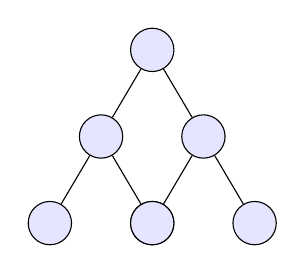
\begin{tikzpicture}[
        level distance=11mm, sibling distance=13mm,
        every node/.style={circle, draw, fill=blue!10, minimum size=5.5mm, font=\scriptsize}
      ]
      \node {}
        child { node {}
          child { node {} }
          child { node {} }
        }
        child { node {}
          child { node {} }
          child { node {} }
        };
    \end{tikzpicture}
    \caption{Level-wise: chia đều tất cả các lá ở mỗi tầng, cây cân đối.}
  \end{subfigure}
  \hfill
  \begin{subfigure}[b]{0.47\textwidth}
    \centering
    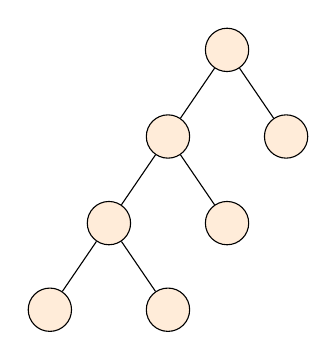
\begin{tikzpicture}[
        level distance=11mm,
        every node/.style={circle, draw, fill=orange!15, minimum size=5.5mm, font=\scriptsize}
      ]
      \node {}
        child { node {}
          child { node {}
            child { node {} }
            child { node {} }
          }
          child { node {} }
        }
        child { node {} };
    \end{tikzpicture}
    \caption{Leaf-wise: luôn chia lá giảm mất mát nhiều nhất, cây bất đối
    xứng.}
  \end{subfigure}
  \caption{So sánh chiến lược tăng trưởng cây level-wise (trái) và leaf-wise
  (phải) với cùng số lá.}
  \label{fig:growth}
\end{figure}

Như minh hoạ ở Hình~\ref{fig:growth}, với cùng số lượng lá, chiến lược
leaf-wise thường đạt mức giảm mất mát lớn hơn level-wise (vì luôn ưu tiên
``điểm nóng'' của sai số), nhưng đổi lại có thể tạo ra cây \textbf{sâu và lệch}
hơn --- dễ học vẹt hơn trên tập dữ liệu nhỏ nếu không kiểm soát chặt các siêu
tham số như \code{num\_leaves}, \code{max\_depth} hay
\code{min\_child\_samples}.

\subsection{GOSS --- Gradient-based One-Side Sampling}

Trực giác của GOSS: những mẫu có \textbf{gradient lớn} (mô hình hiện tại dự
báo sai nhiều) đóng góp nhiều thông tin hơn cho việc tìm điểm chia tốt ở vòng
tiếp theo, trong khi những mẫu có gradient nhỏ (đã được dự báo tốt) đóng góp
ít hơn. GOSS khai thác điều này để giảm số mẫu cần xét khi tìm điểm chia:

\begin{itemize}[leftmargin=*]
  \item Giữ lại \textbf{toàn bộ} $a\%$ số mẫu có gradient (trị tuyệt đối) lớn
        nhất.
  \item Lấy mẫu \textbf{ngẫu nhiên} $b\%$ trong số các mẫu gradient nhỏ còn
        lại.
  \item Để không làm chệch ước lượng độ giảm mất mát (vì đã bỏ bớt mẫu gradient
        nhỏ), gradient của các mẫu được lấy mẫu ngẫu nhiên này được
        \textbf{nhân bù} với hệ số $\frac{1-a}{b}$ khi tính toán thống kê tại
        mỗi điểm chia tiềm năng.
\end{itemize}

Nhờ đó, LightGBM có thể tìm điểm chia gần chính xác như khi dùng toàn bộ dữ
liệu, nhưng chỉ cần xét một tập con nhỏ hơn nhiều --- giảm đáng kể thời gian
huấn luyện trên tập dữ liệu lớn.

\subsection{EFB --- Exclusive Feature Bundling}

Với dữ liệu có nhiều đặc trưng thưa và \textbf{loại trừ lẫn nhau} (mutually
exclusive --- hiếm khi cùng khác 0, điển hình là các đặc trưng one-hot từ mã
hoá biến phân loại nhiều mức), EFB gộp nhiều đặc trưng như vậy thành
\textbf{một} đặc trưng tổng hợp duy nhất, bằng cách gán cho mỗi đặc trưng gốc
một khoảng giá trị riêng biệt trong đặc trưng gộp. Việc xác định nhóm đặc
trưng nào có thể gộp với nhau (cho phép một tỷ lệ xung đột nhỏ, có kiểm soát)
được quy về bài toán \textbf{tô màu đồ thị} (graph coloring) trên đồ thị xung
đột giữa các đặc trưng, giải gần đúng bằng thuật toán tham lam (greedy). Kết
quả là số lượng đặc trưng cần xét khi xây dựng histogram cho việc tìm điểm
chia giảm đáng kể, kéo theo tốc độ huấn luyện nhanh hơn mà hầu như không đánh
đổi độ chính xác.

\subsection{Ưu điểm và hạn chế}

\textbf{Ưu điểm:}
\begin{itemize}[leftmargin=*]
  \item Huấn luyện rất nhanh và tiết kiệm bộ nhớ nhờ GOSS và EFB, phù hợp với
        tập dữ liệu lớn (hàng trăm nghìn bản ghi khi tính theo nhiều mốc thời
        gian).
  \item Chiến lược leaf-wise giúp đạt độ chính xác cao với số lá ít hơn so với
        level-wise.
  \item Nắm bắt tốt quan hệ phi tuyến và tương tác; bền vững với đa cộng tuyến
        và giá trị ngoại lai; tự động xử lý được giá trị thiếu và hỗ trợ trọng
        số lớp để bù mất cân bằng nhãn.
\end{itemize}

\textbf{Hạn chế:}
\begin{itemize}[leftmargin=*]
  \item Dễ học vẹt nếu không tinh chỉnh cẩn thận --- cây leaf-wise có thể phát
        triển sâu và lệch, nhất là khi dữ liệu tại một số mốc thời gian còn
        ít.
  \item Nhạy với việc chọn siêu tham số (đặc biệt \code{num\_leaves} và
        \code{min\_child\_samples}), cần tinh chỉnh kỹ để đạt hiệu quả tốt.
  \item Là mô hình dạng ``hộp đen'', khó diễn giải trực tiếp nếu không dùng
        công cụ bổ trợ.
\end{itemize}

\section{So sánh tổng quan bốn thuật toán}

Bảng~\ref{tab:compare_theory} tổng hợp bốn thuật toán theo các tiêu chí thực
tiễn liên quan trực tiếp đến đặc điểm dữ liệu của bài toán cảnh báo sớm rủi ro
học tập.

\begin{table}[H]
  \centering
  \caption{So sánh đặc điểm lý thuyết của bốn thuật toán.}
  \label{tab:compare_theory}
  \small
  \resizebox{\textwidth}{!}{%
  \begin{tabular}{lllll}
    \toprule
    \textbf{Tiêu chí} & \textbf{LogReg} & \textbf{Random Forest} &
    \textbf{CatBoost} & \textbf{LightGBM} \\
    \midrule
    Kiểu học tập hợp        & Không          & Bagging        & Boosting        & Boosting \\
    Nắm bắt phi tuyến       & Không          & Có             & Có              & Có \\
    Cần chuẩn hoá dữ liệu   & Có             & Không          & Không           & Không \\
    Xử lý đặc trưng phân loại & Cần mã hoá   & Cần mã hoá     & Tự động (Ordered TS) & Tự động (giới hạn) \\
    Xử lý giá trị thiếu     & Không          & Không          & Có              & Có \\
    Bền vững với ngoại lai  & Thấp           & Cao            & Cao             & Cao \\
    Khả năng diễn giải      & Cao            & Trung bình     & Thấp            & Thấp \\
    Tốc độ huấn luyện       & Rất nhanh      & Trung bình     & Chậm nhất       & Nhanh nhất \\
    Tốc độ dự báo           & Rất nhanh      & Trung bình     & Rất nhanh       & Nhanh \\
    Nguy cơ học vẹt         & Thấp           & Trung bình     & Thấp (Ordered Boosting) & Trung bình--cao (leaf-wise) \\
    \bottomrule
  \end{tabular}}
\end{table}

\section{Kết luận}

Bốn thuật toán trình bày ở trên bổ khuyết cho nhau về mặt lý thuyết: Logistic
Regression cung cấp một mô hình cơ sở đơn giản, nhanh và dễ diễn giải nhưng bị
giới hạn bởi giả định tuyến tính; Random Forest và hai thuật toán boosting
(CatBoost, LightGBM) đều dựa trên cây quyết định nên tự nhiên nắm bắt được
quan hệ phi tuyến và tương tác giữa các đặc trưng --- đặc điểm đã được xác
nhận là tồn tại rõ trong dữ liệu ở giai đoạn phân tích khám phá --- nhưng khác
biệt về cơ chế tổng hợp (song song vs.\ tuần tự) và do đó có đặc tính bias--variance
khác nhau. Trong hai thuật toán boosting, CatBoost ưu tiên xử lý đặc trưng
phân loại và giảm rò rỉ mục tiêu một cách nguyên bản, còn LightGBM ưu tiên tốc
độ và khả năng mở rộng trên dữ liệu lớn. Việc đưa đồng thời cả bốn thuật toán
vào thực nghiệm, như trình bày ở báo cáo xây dựng và so sánh mô hình, cho phép
đối chiếu trực tiếp những đánh đổi lý thuyết này trên chính dữ liệu của bài
toán cảnh báo sớm rủi ro học tập.

\end{document}
